\documentclass[11pt]{article}

\usepackage[a4paper, margin=1in]{geometry}
\usepackage{graphicx}
\usepackage{hyperref}
\usepackage{longtable}
\usepackage{array}
\usepackage{enumitem}
\usepackage{xcolor}
\usepackage{titlesec}
\usepackage{booktabs}
\usepackage{tabularx}
\usepackage{fancyhdr}
\usepackage{tikz}
\usetikzlibrary{arrows.meta, positioning, shapes, calc}
\usetikzlibrary{shapes.geometric, shapes.misc, backgrounds, fit, arrows.meta}


\hypersetup{
    colorlinks=true,
    linkcolor=black,
    urlcolor=blue,
    citecolor=black
}

\definecolor{cmuRed}{HTML}{C41230}
\definecolor{phaseOne}{HTML}{DBEAFE}
\definecolor{phaseTwo}{HTML}{D1FAE5}
\definecolor{phaseThree}{HTML}{FFE4E6}
\definecolor{phaseFour}{HTML}{FEF3C7}
\definecolor{sectionGray}{HTML}{F1F3F5}
\definecolor{deferGray}{HTML}{E5E7EB}

\titleformat{\section}{\Large\bfseries\color{cmuRed}}{}{0em}{}[\vspace{0.2em}\titlerule]
\titleformat{\subsection}{\large\bfseries}{}{0em}{}
\titleformat{\subsubsection}{\normalsize\bfseries}{}{0em}{}

\pagestyle{fancy}
\fancyhf{}
\fancyhead[L]{\textcolor{cmuRed}{\textbf{CountsFor}} — Sprint 1 Plan}
\fancyhead[R]{\textcolor{gray}{CMU-Q · April 2026}}
\fancyfoot[C]{\thepage}
\renewcommand{\headrulewidth}{0.4pt}

\begin{document}

% ============================================================
% TITLE PAGE
% ============================================================
\begin{titlepage}
\centering
\vspace*{2cm}

{\Huge\bfseries\textcolor{cmuRed}{CountsFor}}\\[0.5cm]
{\LARGE Sprint 1 — Foundation Plan}\\[0.3cm]
{\large UI/UX Redesign \& Backend Integration}\\[1.5cm]

\rule{0.6\textwidth}{0.4pt}\\[1cm]

{\large
\textbf{Authors}\\[0.4cm]
Aditya Vivek\\
\textit{Frontend Developer}\\[0.3cm]
Hind Jendara\\
\textit{Backend Developer}\\[0.8cm]
}

{\large Carnegie Mellon University in Qatar}\\[0.3cm]
{\normalsize April 4, 2026}\\[1.5cm]

\rule{0.6\textwidth}{0.4pt}\\[1cm]

{\normalsize
\textbf{Project Repository:} \url{https://github.com/Adicmu/Countsfor-Summer-26}\\[0.2cm]
\textbf{Live Site:} \url{https://countsfor.qatar.cmu.edu}\\[0.2cm]
\textbf{Sprint Duration:} April 5 -- April 23, 2026\\[0.2cm]
\textbf{Time Budget:} $\sim$30 hours total (10 hrs/week $\times$ 3 weeks)
}

\vfill
{\small Version 1.1 — Updated Time Budget}
\end{titlepage}

% ============================================================
\tableofcontents
\newpage

% ============================================================
\section{Executive Summary}

This document outlines \textbf{Sprint 1} of the CountsFor redesign project, running from \textbf{April 5--23, 2026}. Given a constraint of \textbf{10 hours per week per person} ($\sim$30 total hours each, $\sim$60 combined hours), this sprint is scoped to deliver the highest-impact improvements:

\begin{enumerate}[label=\textbf{\arabic*.}]
    \item \textbf{Frontend (Aditya):} Establish the new project scaffold and design system, build a modern navigation shell (slim navbar, unified filter bar, footer), apply the new visual language to the course table, and add a dark mode toggle.
    \item \textbf{Backend (Hind):} Set up the PostgreSQL database, migrate all existing course data, stand up core API endpoints, and wire them to the frontend for live data retrieval and functional filtering.
\end{enumerate}

\noindent
\textbf{Guiding Principle:} By April 23, a student visiting CountsFor should see a \textit{noticeably modernized} interface where the core filters and ``Add to Plan'' buttons actually work against live data. Advanced features (full mobile card layout, onboarding tour, analytics overhaul, semester auto-updates, full WCAG audit) are explicitly \textbf{deferred to Sprint 2+} in the summer.

% ============================================================
\section{Constraints \& Scoping}

\subsection{Time Budget}

\begin{tabular}{p{0.35\textwidth} p{0.55\textwidth}}
\toprule
\textbf{Constraint} & \textbf{Value} \\
\midrule
Hours per week & 10 hours/person \\
Sprint duration & 3 weeks (April 5--23) \\
Total hours per person & $\sim$30 hours \\
Combined team hours & $\sim$60 hours \\
Working days & $\sim$15 effective working days \\
\bottomrule
\end{tabular}

\subsection{What's IN Sprint 1 vs. Deferred}

\begin{longtable}{p{0.38\textwidth} p{0.12\textwidth} p{0.12\textwidth} p{0.25\textwidth}}
\toprule
\textbf{Feature} & \textbf{Sprint 1?} & \textbf{Est.\ Hours} & \textbf{Notes} \\
\midrule
Next.js scaffold + Tailwind setup & \textcolor{green!60!black}{\textbf{Yes}} & 4h & Foundation \\
Design tokens (colors, fonts) & \textcolor{green!60!black}{\textbf{Yes}} & 3h & Carnegie Red palette \\
Slim sticky navbar & \textcolor{green!60!black}{\textbf{Yes}} & 4h & Replace oversized hero \\
Unified filter bar (desktop) & \textcolor{green!60!black}{\textbf{Yes}} & 4h & Clean dropdown row \\
Branded footer & \textcolor{green!60!black}{\textbf{Yes}} & 2h & Quick win \\
Basic dark mode toggle & \textcolor{green!60!black}{\textbf{Yes}} & 3h & Light/dark with persistence \\
Course table restyling (muted colors) & \textcolor{green!60!black}{\textbf{Yes}} & 5h & Pills + muted accents \\
Basic responsive cleanup & \textcolor{green!60!black}{\textbf{Yes}} & 3h & No broken layouts \\
PostgreSQL schema + setup & \textcolor{green!60!black}{\textbf{Yes}} & 4h & 7 core tables \\
Data migration script & \textcolor{green!60!black}{\textbf{Yes}} & 5h & Seed 595+ courses \\
FastAPI core endpoints & \textcolor{green!60!black}{\textbf{Yes}} & 5h & Courses, majors, buckets \\
Wire filters to API & \textcolor{green!60!black}{\textbf{Yes}} & 4h & Functional dropdowns \\
Add to Plan button (basic) & \textcolor{green!60!black}{\textbf{Yes}} & 4h & Per-row + localStorage \\
Basic sort by column & \textcolor{green!60!black}{\textbf{Yes}} & 3h & Click header to sort \\
Integration smoke test & \textcolor{green!60!black}{\textbf{Yes}} & 3h & Core flows work \\
\midrule
\rowcolor{deferGray}
Full mobile card layout & Deferred & --- & Sprint 2 \\
\rowcolor{deferGray}
Framer Motion animations & Deferred & --- & Sprint 2 \\
\rowcolor{deferGray}
Full WCAG accessibility audit & Deferred & --- & Sprint 2 \\
\rowcolor{deferGray}
Expandable prerequisite rows & Deferred & --- & Sprint 2 \\
\rowcolor{deferGray}
Onboarding tooltip tour & Deferred & --- & Sprint 2 \\
\rowcolor{deferGray}
Analytics tab redesign & Deferred & --- & Sprint 3 \\
\rowcolor{deferGray}
Semester auto-update pipeline & Deferred & --- & Sprint 3 \\
\rowcolor{deferGray}
Fuse.js fuzzy search & Deferred & --- & Sprint 2 \\
\rowcolor{deferGray}
Virtual scrolling (react-virtual) & Deferred & --- & Sprint 2 \\
\rowcolor{deferGray}
Docker deployment & Deferred & --- & Sprint 2 \\
\rowcolor{deferGray}
Plan tab grouping by major & Deferred & --- & Sprint 2 \\
\bottomrule
\end{longtable}

\textbf{Total estimated hours (Sprint 1):} $\sim$56h combined ($\sim$28h Aditya, $\sim$22h Hind, $\sim$6h shared).\\
This leaves $\sim$4 hours of buffer for debugging, communication, and unexpected issues.

% ============================================================
\section{Current State Assessment}

\subsection{Technology Stack (As-Is)}

\begin{tabular}{p{0.25\textwidth} p{0.65\textwidth}}
\toprule
\textbf{Layer} & \textbf{Current Technology} \\
\midrule
Framework & React (Create React App) \\
Styling & Inline styles + single CSS file \\
Data & Static/hardcoded JSON within the React bundle \\
Hosting & CMU-Q infrastructure (\texttt{countsfor.qatar.cmu.edu}) \\
\bottomrule
\end{tabular}

\subsection{Key Problems This Sprint Addresses}

\begin{tabular}{p{0.05\textwidth} p{0.3\textwidth} p{0.15\textwidth} p{0.38\textwidth}}
\toprule
\textbf{\#} & \textbf{Problem} & \textbf{Severity} & \textbf{Sprint 1 Action} \\
\midrule
1 & Oversized hero (20\% viewport) & High & Replace with slim 56px navbar \\
2 & Saturated color columns & High & Muted accent palette \\
3 & No dark mode & Medium & Light/dark toggle \\
4 & Cluttered filter dropdowns & High & Unified filter bar \\
5 & Buttons don't work (Add to Plan, Sort) & Critical & Wire to state + API \\
6 & No dynamic data retrieval & Critical & PostgreSQL + FastAPI \\
7 & No footer branding & Low & Branded footer \\
8 & Inconsistent typography & Medium & Inter + JetBrains Mono \\
\bottomrule
\end{tabular}

% ============================================================
\section{Target Technology Stack}

\begin{tabular}{p{0.2\textwidth} p{0.25\textwidth} p{0.45\textwidth}}
\toprule
\textbf{Layer} & \textbf{Technology} & \textbf{Rationale} \\
\midrule
Framework & Next.js 14+ & App Router, SSR capability \\
Styling & Tailwind CSS v4 & Utility-first, built-in dark mode \\
Components & shadcn/ui & Accessible Radix-based primitives \\
Data Fetching & TanStack Query v5 & Caching + background refetch \\
State & Zustand & Lightweight client state (plan) \\
Charts & Recharts & Responsive charts (Sprint 2) \\
API & FastAPI (Python) & Read-only REST endpoints \\
Database & PostgreSQL & Structured course/bucket storage \\
\bottomrule
\end{tabular}

% ============================================================
\section{Architecture Overview}

\begin{figure}[h!]
\centering
\resizebox{0.92\textwidth}{!}{%
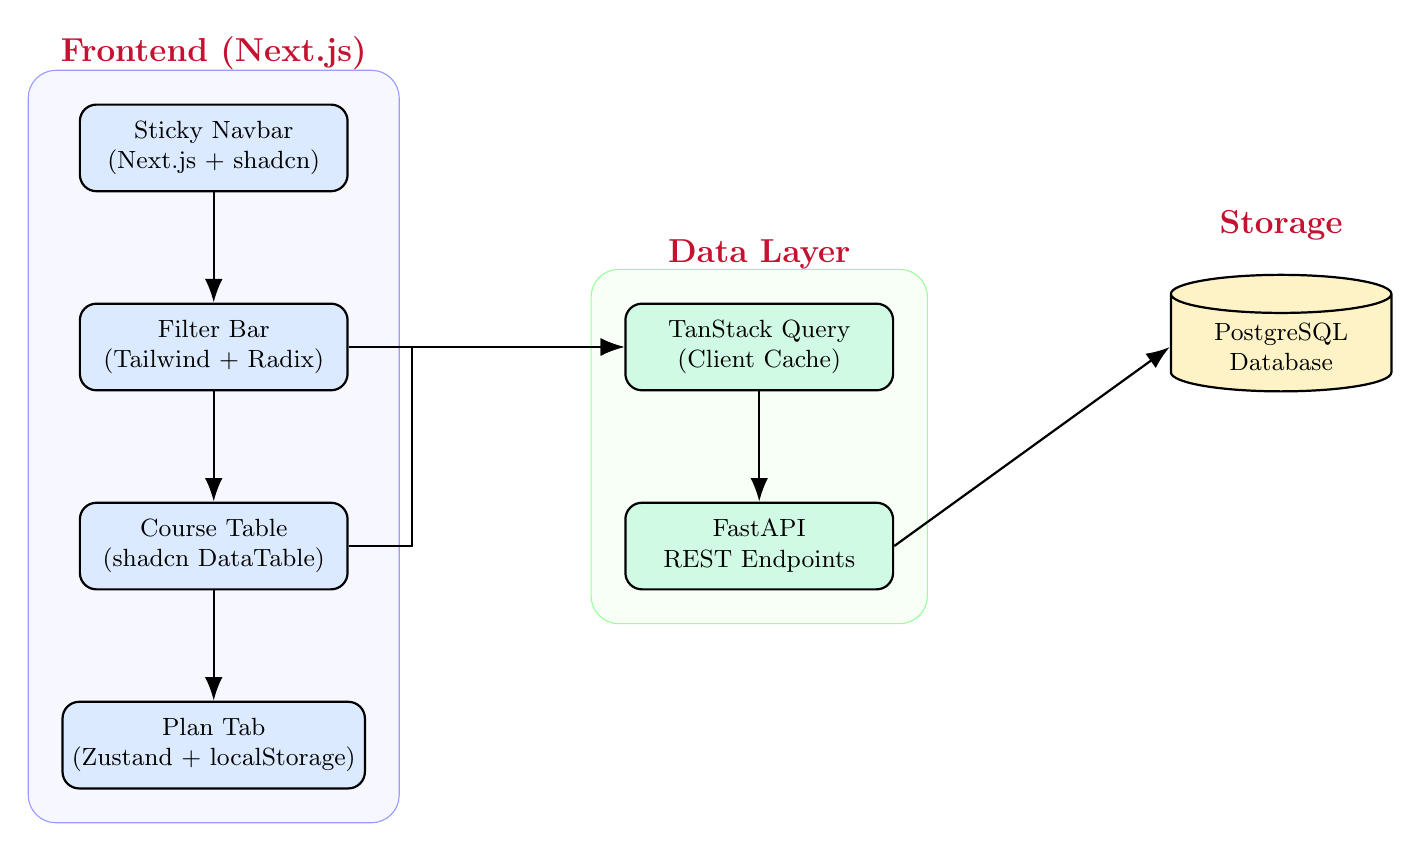
\begin{tikzpicture}[
    node distance=1.4cm and 2.2cm,
    every node/.style={font=\small},
    box/.style={
        rectangle, draw=black, rounded corners=6pt,
        minimum width=3.4cm, minimum height=1.1cm,
        align=center, thick
    },
    frontbox/.style={box, fill=phaseOne},
    apibox/.style={box, fill=phaseTwo},
    dbbox/.style={
        cylinder, shape= cylinder, draw=black, shape border rotate=90,
        aspect=0.25, fill=phaseFour, align=center,
        minimum height=1.3cm, minimum width=2.8cm, thick
    },
    arrow/.style={-{Latex[length=3mm]}, thick}
]

\node[frontbox] (navbar) {Sticky Navbar\\(Next.js + shadcn)};
\node[frontbox, below=of navbar] (filters) {Filter Bar\\(Tailwind + Radix)};
\node[frontbox, below=of filters] (table) {Course Table\\(shadcn DataTable)};
\node[frontbox, below=of table] (plan) {Plan Tab\\(Zustand + localStorage)};

\node[apibox, right=3.5cm of filters] (tanstack) {TanStack Query\\(Client Cache)};
\node[apibox, below=of tanstack] (api) {FastAPI\\REST Endpoints};

\node[dbbox, right=3.5cm of tanstack] (db) {PostgreSQL\\Database};

\node[above=0.3cm of navbar, font=\bfseries\large, color=cmuRed] {Frontend (Next.js)};
\node[above=0.3cm of tanstack, font=\bfseries\large, color=cmuRed] {Data Layer};
\node[above=0.3cm of db, font=\bfseries\large, color=cmuRed] {Storage};

\draw[arrow] (navbar) -- (filters);
\draw[arrow] (filters) -- (table);
\draw[arrow] (table) -- (plan);
\draw[arrow] (filters.east) -- ++(0.8,0) |- (tanstack.west);
\draw[arrow] (table.east) -- ++(0.8,0) |- (tanstack.west);
\draw[arrow] (tanstack) -- (api);
\draw[arrow] (api.east) -- (db.west);

\begin{scope}[on background layer]
    \node[draw=blue!40, fill=blue!3, rounded corners=10pt,
          fit=(navbar)(filters)(table)(plan),
          inner sep=12pt] {};
    \node[draw=green!40, fill=green!3, rounded corners=10pt,
          fit=(tanstack)(api),
          inner sep=12pt] {};
\end{scope}

\end{tikzpicture}
}
\caption{Sprint 1 Architecture — Frontend $\leftrightarrow$ API $\leftrightarrow$ Database}
\end{figure}

% ============================================================
\section{Sprint Plan — 5 Phases Over $\sim$19 Days}

\subsection{Phase Overview}

\begin{figure}[h!]
\centering
\resizebox{\textwidth}{!}{%
\begin{tabular}{|c|c|c|l|c|c|}
\hline
\rowcolor{sectionGray}
\textbf{Phase} & \textbf{Days} & \textbf{Est.\ Hours} & \textbf{Focus Area} & \textbf{Owner} & \textbf{Deliverable} \\
\hline
\rowcolor{phaseOne}
1 & 1--4 & 10h (A) & Design System + Page Shell & Aditya & Scaffold + navbar + filters + footer \\
\hline
\rowcolor{phaseTwo}
2 & 1--6 & 14h (H) & Database + API & Hind & PostgreSQL schema + FastAPI endpoints \\
\hline
\rowcolor{phaseThree}
3 & 5--10 & 8h (A) & Course Table + Dark Mode & Aditya & Restyled table + theme toggle \\
\hline
\rowcolor{phaseFour}
4 & 7--14 & 12h (A+H) & Wiring: Filters, Sort, Plan & Both & Functional buttons + live data \\
\hline
\rowcolor{sectionGray}
5 & 15--19 & 6h (A+H) & Testing + Polish & Both & Smoke test + bug fixes \\
\hline
\end{tabular}
}
\caption{Sprint 1 Phases — A = Aditya, H = Hind. Phases 1 \& 2 run in parallel.}
\end{figure}

\noindent
\textit{Note: Aditya and Hind work in parallel during the first week. Phases 1 (frontend) and 2 (backend) overlap, so both developers are productive from Day 1.}

\newpage

% ============================================================
\subsection{Phase 1: Design System + Page Shell (Days 1--4)}

\textbf{Owner:} Aditya Vivek \hfill \textbf{Estimated:} 10 hours

\subsubsection{Day 1--2: Project Scaffold \& Design Tokens ($\sim$5h)}

\begin{itemize}[leftmargin=2em]
    \item Initialize Next.js 14+ with App Router, Tailwind CSS v4, shadcn/ui
    \item Set up project structure:
    \begin{verbatim}
    src/
      app/
        layout.tsx        # Root layout
        page.tsx          # View tab (default)
        plan/page.tsx     # Plan tab
        analytics/page.tsx
      components/
        ui/               # shadcn primitives
        layout/           # Navbar, Footer, FilterBar
        course/           # CourseTable, CourseRow
      lib/
        api.ts            # TanStack Query hooks
        store.ts          # Zustand store
      styles/
        globals.css       # Tailwind + CSS variables
    \end{verbatim}
    \item Define CSS custom properties — full color palette:
    \begin{itemize}
        \item Primary: Carnegie Red (\texttt{\#C41230})
        \item Background: \texttt{\#FAFBFC} (light) / \texttt{\#0F172A} (dark)
        \item Surface: \texttt{\#F1F3F5} (light) / \texttt{\#1E293B} (dark)
        \item Muted major accents: BA Blue, BS Green, CS Rose, IS Amber
    \end{itemize}
    \item Configure Google Fonts: \textbf{Inter} (UI) + \textbf{JetBrains Mono} (course codes)
    \item Install shadcn components: Button, Badge, Select, Tabs, Table, Switch, Sheet
    \item Push scaffold to GitHub
\end{itemize}

\subsubsection{Days 3--4: Navbar, Filter Bar \& Footer ($\sim$5h)}

\begin{itemize}[leftmargin=2em]
    \item \texttt{<Navbar>} — 56px height, sticky, frosted-glass backdrop-blur:
    \begin{itemize}
        \item Left: ``CountsFor'' wordmark (Carnegie Red)
        \item Center: View $|$ Plan $|$ Analytics tabs (active underline indicator)
        \item Right: Dark mode toggle icon
    \end{itemize}
    \item \texttt{<FilterBar>} — single-row card below navbar:
    \begin{itemize}
        \item Search input (left) with magnifying glass icon, debounced 300ms
        \item Department dropdown (shadcn Select)
        \item Location dropdown (Qatar / Pittsburgh)
        \item Course Type dropdown
        \item ``Clear All'' ghost button (right)
        \item Result count: ``Showing X of Y courses''
    \end{itemize}
    \item \texttt{<Footer>} — branded:
    \begin{itemize}
        \item Carnegie Red accent line at top
        \item ``\textcopyright\ 2026 Carnegie Mellon University in Qatar''
        \item ``Last Updated'' placeholder (will connect to \texttt{/api/status} later)
    \end{itemize}
    \item Wire tab routing: \texttt{/} $\rightarrow$ View, \texttt{/plan} $\rightarrow$ Plan, \texttt{/analytics} $\rightarrow$ Analytics
\end{itemize}

\noindent
\textbf{Checkpoint:} Full page shell visible — slim navbar, filter bar, empty content area, footer. Navigation between tabs works.

\noindent\rule{\textwidth}{0.2pt}

% ============================================================
\subsection{Phase 2: Database + API (Days 1--6)}

\textbf{Owner:} Hind Jendara \hfill \textbf{Estimated:} 14 hours\\
\textit{Runs in parallel with Phase 1.}

\subsubsection{Days 1--2: PostgreSQL Schema ($\sim$4h)}

\begin{itemize}[leftmargin=2em]
    \item Set up PostgreSQL (local Docker or CMU-Q VM)
    \item Create schema — 7 tables:
    
    \begin{verbatim}
    courses        (course_id PK, title, units, department, location)
    semesters      (semester_id PK, name, is_current)
    offerings      (semester_id FK, course_id FK, offered)
    majors         (major_code PK, major_name)
    buckets        (bucket_id, major_code FK, bucket_name)
    course_bucket_map (course_id FK, major_code, bucket_id)
    prerequisites  (course_id FK, prereq_text)
    \end{verbatim}
    
    \item Create indexes on \texttt{course\_id}, \texttt{major\_code}, \texttt{semester\_id}
\end{itemize}

\subsubsection{Days 3--4: Data Migration ($\sim$5h)}

\begin{itemize}[leftmargin=2em]
    \item Extract course data from the existing React app's static bundle
    \item Write \texttt{scripts/seed\_db.py}:
    \begin{itemize}
        \item Parse existing course JSON/JS data
        \item Map courses $\rightarrow$ BA/BS/CS/IS buckets
        \item Insert offering history (semester codes like F24, S25)
        \item Insert prerequisite text
    \end{itemize}
    \item Validate: all 595+ courses present, bucket mappings correct
\end{itemize}

\subsubsection{Days 5--6: FastAPI Endpoints ($\sim$5h)}

\begin{itemize}[leftmargin=2em]
    \item Set up FastAPI project:
    \begin{verbatim}
    api/
      main.py           # App + CORS config
      routers/courses.py
      routers/majors.py
      routers/status.py
      models/schemas.py  # Pydantic models
      db/connection.py   # SQLAlchemy
    \end{verbatim}
    
    \item Implement endpoints:
    
    \begin{tabular}{p{0.10\textwidth} p{0.40\textwidth} p{0.38\textwidth}}
    \toprule
    \textbf{Method} & \textbf{Endpoint} & \textbf{Description} \\
    \midrule
    GET & \texttt{/api/courses} & All courses; supports \texttt{?search}, \texttt{?department}, \texttt{?location}, \texttt{?type} \\
    GET & \texttt{/api/courses/\{id\}} & Single course with full details \\
    GET & \texttt{/api/majors} & List of majors \\
    GET & \texttt{/api/majors/\{code\}/buckets} & Buckets for a major \\
    GET & \texttt{/api/semesters} & Available semesters \\
    GET & \texttt{/api/status} & Last updated timestamp \\
    \bottomrule
    \end{tabular}
    
    \item Configure CORS for \texttt{countsfor.qatar.cmu.edu} + \texttt{localhost:3000}
    \item Test via Swagger UI (\texttt{/docs})
\end{itemize}

\noindent
\textbf{Checkpoint:} All API endpoints return correct data. Swagger UI shows valid responses. Database contains all 595+ courses with correct bucket mappings.

\noindent\rule{\textwidth}{0.2pt}

% ============================================================
\subsection{Phase 3: Course Table + Dark Mode (Days 5--10)}

\textbf{Owner:} Aditya Vivek \hfill \textbf{Estimated:} 8 hours

\subsubsection{Days 5--7: Course Table Restyling ($\sim$5h)}

\begin{itemize}[leftmargin=2em]
    \item Replace the current saturated color columns with muted accent system:
    \begin{itemize}
        \item BA: \texttt{bg-blue-50/60} (light) / \texttt{bg-blue-950/20} (dark)
        \item BS: \texttt{bg-emerald-50/60} / \texttt{bg-emerald-950/20}
        \item CS: \texttt{bg-rose-50/60} / \texttt{bg-rose-950/20}
        \item IS: \texttt{bg-amber-50/60} / \texttt{bg-amber-950/20}
    \end{itemize}
    \item Redesign table headers:
    \begin{itemize}
        \item Sticky below navbar
        \item Major name + colored dot indicator
        \item 13px Inter SemiBold, uppercase, letter-spaced
    \end{itemize}
    \item Redesign cells:
    \begin{itemize}
        \item Requirement text as \texttt{<Badge>} pill components instead of bullet lists
        \item Hover row highlight
        \item Alternating row backgrounds
    \end{itemize}
    \item Course code column: JetBrains Mono font
    \item ``Offered'' column: semester codes as small pill badges
    \item Ensure basic horizontal scroll on narrow screens (no broken layout)
\end{itemize}

\subsubsection{Days 8--10: Dark Mode ($\sim$3h)}

\begin{itemize}[leftmargin=2em]
    \item Install \texttt{next-themes} for theme management
    \item Implement dark mode toggle in navbar (Sun/Moon icon):
    \begin{itemize}
        \item Auto-detect \texttt{prefers-color-scheme}
        \item Persist choice in \texttt{localStorage}
    \end{itemize}
    \item Dark mode color mapping:
    \begin{itemize}
        \item Background: \texttt{\#0F172A}, Surface: \texttt{\#1E293B}
        \item Text: \texttt{\#F1F5F9} primary, \texttt{\#94A3B8} secondary
        \item Major accents at 15\% opacity
        \item Borders: \texttt{\#334155}
    \end{itemize}
    \item Verify all shadcn components respect \texttt{.dark} class
    \item Quick contrast check on text readability
\end{itemize}

\noindent
\textbf{Checkpoint:} Course table has modern styling with muted colors and pill badges. Dark mode toggles cleanly. No visual regressions.

\noindent\rule{\textwidth}{0.2pt}

% ============================================================
\subsection{Phase 4: Wiring — Filters, Sort, Add to Plan (Days 7--14)}

\textbf{Owner:} Aditya (frontend wiring) + Hind (API support) \hfill \textbf{Estimated:} 12 hours

\subsubsection{Days 7--9: Connect Frontend to API ($\sim$5h)}

\begin{itemize}[leftmargin=2em]
    \item Install TanStack Query v5, set up \texttt{QueryClientProvider}
    \item Create hooks:
    \begin{itemize}
        \item \texttt{useCourses(filters)} $\rightarrow$ \texttt{GET /api/courses?...}
        \item \texttt{useMajors()} $\rightarrow$ \texttt{GET /api/majors}
        \item \texttt{useBuckets(majorCode)} $\rightarrow$ \texttt{GET /api/majors/\{code\}/buckets}
    \end{itemize}
    \item Replace all hardcoded data with API calls
    \item Add loading spinner while data fetches
    \item Add simple error state with ``Retry'' button
\end{itemize}

\subsubsection{Days 10--12: Functional Filters + Sort ($\sim$4h)}

\begin{itemize}[leftmargin=2em]
    \item Wire filter bar to API query parameters:
    \begin{itemize}
        \item Department $\rightarrow$ \texttt{?department=X}
        \item Location $\rightarrow$ \texttt{?location=Qatar|Pittsburgh}
        \item Course Type $\rightarrow$ \texttt{?type=Core|GenEd}
        \item Search $\rightarrow$ \texttt{?search=X} (debounced)
    \end{itemize}
    \item ``Clear All Filters'' resets state and refetches
    \item Column header click $\rightarrow$ sorts table (client-side):
    \begin{itemize}
        \item Sort by Course Code, Title, or Offered
        \item Arrow icon toggles asc/desc
    \end{itemize}
    \item ``Sort by Requirements Met'' — counts non-empty bucket mappings per course, sorts descending
\end{itemize}

\subsubsection{Days 12--14: Add to Plan + Plan Tab ($\sim$3h)}

\begin{itemize}[leftmargin=2em]
    \item Zustand store for plan: \texttt{\{planCourses, addCourse, removeCourse, clearPlan\}}
    \item Persist plan to \texttt{localStorage}
    \item Per-row ``+ Add'' button:
    \begin{itemize}
        \item Changes to ``$\checkmark$ Added'' (green) when course is in plan
        \item Click again to remove
    \end{itemize}
    \item Plan tab (\texttt{/plan}):
    \begin{itemize}
        \item Simple list of added courses (code, title, units)
        \item Total units count at top
        \item ``Remove'' button per row
        \item ``Clear Plan'' button
    \end{itemize}
\end{itemize}

\noindent
\textbf{Checkpoint:} Filters narrow the course list via live API. Sorting works. ``Add to Plan'' persists across refresh. Plan tab shows selections.

\noindent\rule{\textwidth}{0.2pt}

% ============================================================
\subsection{Phase 5: Testing + Polish (Days 15--19)}

\textbf{Owner:} Both \hfill \textbf{Estimated:} 6 hours

\subsubsection{Days 15--17: Smoke Testing ($\sim$3h)}

Core flow checklist:

\begin{itemize}[leftmargin=2em]
    \item[$\square$] Page loads and displays courses from API
    \item[$\square$] Department filter returns correct results
    \item[$\square$] Location filter works (Qatar / Pittsburgh)
    \item[$\square$] Search finds courses by code and title
    \item[$\square$] ``Clear All Filters'' resets everything
    \item[$\square$] Column sorting works (asc/desc)
    \item[$\square$] ``Sort by Requirements Met'' orders correctly
    \item[$\square$] ``Add to Plan'' adds course, button changes state
    \item[$\square$] Plan persists across page refresh
    \item[$\square$] Plan tab shows added courses with remove option
    \item[$\square$] Dark mode toggles correctly
    \item[$\square$] No console errors
    \item[$\square$] Navbar tab navigation works
\end{itemize}

\subsubsection{Days 18--19: Bug Fixes + Final Polish ($\sim$3h)}

\begin{itemize}[leftmargin=2em]
    \item Fix all bugs found during testing
    \item Ensure no visual inconsistencies between light/dark mode
    \item Clean up code, remove \texttt{console.log} statements
    \item Push final code to GitHub
    \item Tag release: \texttt{v0.1.0-sprint1}
    \item Update \texttt{README.md} with setup instructions:
    \begin{itemize}
        \item Prerequisites (Node.js 18+, Python 3.11+, PostgreSQL)
        \item \texttt{npm install \&\& npm run dev} (frontend)
        \item \texttt{pip install -r requirements.txt \&\& uvicorn api.main:app} (backend)
        \item Database seeding: \texttt{python scripts/seed\_db.py}
    \end{itemize}
\end{itemize}

% ============================================================
\section{Responsibility Matrix}

\begin{longtable}{p{0.3\textwidth} p{0.10\textwidth} p{0.10\textwidth} p{0.12\textwidth} p{0.2\textwidth}}
\toprule
\textbf{Task} & \textbf{Aditya} & \textbf{Hind} & \textbf{Est.\ Hours} & \textbf{Phase} \\
\midrule
Next.js scaffold + Tailwind & Lead & --- & 4h & Phase 1 \\
Design tokens + typography & Lead & --- & 3h & Phase 1 \\
Navbar component & Lead & --- & 2h & Phase 1 \\
Filter bar component & Lead & --- & 2h & Phase 1 \\
Footer component & Lead & --- & 1h & Phase 1 \\
\midrule
PostgreSQL schema & --- & Lead & 4h & Phase 2 \\
Data migration script & --- & Lead & 5h & Phase 2 \\
FastAPI endpoints & --- & Lead & 5h & Phase 2 \\
\midrule
Course table restyling & Lead & --- & 5h & Phase 3 \\
Dark mode toggle & Lead & --- & 3h & Phase 3 \\
\midrule
TanStack Query hooks & Lead & Support & 4h & Phase 4 \\
Filter wiring to API & Lead & Support & 2h & Phase 4 \\
Sort functionality & Lead & --- & 2h & Phase 4 \\
Add to Plan + Plan tab & Lead & --- & 3h & Phase 4 \\
\midrule
Smoke testing & Lead & Lead & 3h & Phase 5 \\
Bug fixes + polish & Lead & Lead & 3h & Phase 5 \\
\bottomrule
\end{longtable}

\textbf{Totals:} Aditya $\sim$31h, Hind $\sim$21h, Shared $\sim$6h = \textbf{$\sim$58h combined}. Buffer: $\sim$2h.

% ============================================================
\section{Risk Assessment}

\begin{longtable}{p{0.24\textwidth} p{0.12\textwidth} p{0.12\textwidth} p{0.38\textwidth}}
\toprule
\textbf{Risk} & \textbf{Likelihood} & \textbf{Impact} & \textbf{Mitigation} \\
\midrule
Data extraction from CRA bundle fails & Medium & High & Scrape live site as fallback; manually verify key data points \\
CMU-Q VM not available in time & Medium & High & Develop locally with Docker; deploy when VM is ready \\
CORS issues frontend $\leftrightarrow$ API & High & Low & Configure in Day 5; test early with localhost \\
Time overrun on data migration & Medium & Medium & Prioritize core tables (courses, buckets); defer offering history if needed \\
Scope creep & High & Medium & Strict deferral list above; say no to anything not on the Sprint 1 list \\
\bottomrule
\end{longtable}

% ============================================================
\section{Definition of Done — Sprint 1}

By \textbf{April 23, 2026}, the following must be true:

\begin{enumerate}[label=\textbf{\arabic*.}]
    \item \textbf{Visual:} CountsFor has a modern UI with slim sticky navbar, muted accent table columns, Inter + JetBrains Mono typography, branded footer, and a clean filter bar.
    \item \textbf{Dark Mode:} Light/dark toggle works and persists across sessions.
    \item \textbf{Filters Work:} Department, Location, Course Type, and Search all narrow the course list via API queries.
    \item \textbf{Sorting Works:} Column header sorting and ``Sort by Requirements Met'' function correctly.
    \item \textbf{Add to Plan Works:} Per-row add/remove buttons function. Plan persists in localStorage. Plan tab shows selected courses.
    \item \textbf{Data is Live:} Course data is served from PostgreSQL via FastAPI — no hardcoded data in the frontend.
    \item \textbf{No Major Bugs:} All 13 smoke test items pass.
    \item \textbf{Code on GitHub:} Clean commit history, tagged \texttt{v0.1.0-sprint1}, with setup instructions in README.
\end{enumerate}

% ============================================================
\section{Explicitly Deferred to Sprint 2+ (Summer)}

The following are \textbf{out of scope} for Sprint 1 and will be addressed during the full summer engagement:

\begin{longtable}{p{0.35\textwidth} p{0.15\textwidth} p{0.38\textwidth}}
\toprule
\textbf{Feature} & \textbf{Target Sprint} & \textbf{Notes} \\
\midrule
Full mobile card layout & Sprint 2 & Replace table with cards on $<$640px \\
Framer Motion animations & Sprint 2 & Page transitions, micro-interactions \\
Full WCAG 2.1 AA audit & Sprint 2 & axe-core, keyboard nav, screen reader testing \\
Expandable prerequisite rows & Sprint 2 & Click-to-expand with full prereq chain \\
Fuse.js fuzzy search & Sprint 2 & Client-side instant search \\
Virtual scrolling & Sprint 2 & react-virtual for 595+ row performance \\
Plan tab — group by major & Sprint 2 & Visual grouping with unit subtotals \\
Onboarding tooltip tour & Sprint 2 & First-time user guidance \\
Analytics tab redesign & Sprint 3 & Bento-grid dashboard, responsive charts \\
Semester auto-update pipeline & Sprint 3 & Cron job + Registrar CSV ingestion \\
Docker deployment & Sprint 2 & Containerized API + DB \\
Export Plan to PDF/CSV & Sprint 3 & Download plan for advising meetings \\
User authentication & Sprint 3 & Saved plans across devices \\
PWA support & Sprint 3 & Offline access, install prompt \\
\bottomrule
\end{longtable}

% ============================================================
\section{Communication \& Workflow}

\begin{itemize}
    \item \textbf{Repository:} \url{https://github.com/Adicmu/Countsfor-Summer-26}
    \item \textbf{Branching:}
    \begin{itemize}
        \item \texttt{main} — production-ready
        \item \texttt{develop} — integration branch
        \item \texttt{feature/*} — individual branches (e.g., \texttt{feature/navbar}, \texttt{feature/api-courses})
    \end{itemize}
    \item \textbf{Check-ins:} Quick async update 2--3x per week on progress/blockers
    \item \textbf{Mid-Sprint Check (Day 8--9):} Frontend shell + API both independently working
    \item \textbf{End-Sprint Demo (Day 19):} Full integrated demo
\end{itemize}

\vspace{1cm}
\noindent\rule{\textwidth}{0.4pt}
\begin{center}
\textit{Prepared by Aditya Vivek \& Hind Jendara}\\
\textit{Carnegie Mellon University in Qatar}\\
\textit{April 2026}
\end{center}

\end{document}
